
%%%%%%%%%%%%%%%%%%%%%%% file typeinst.tex %%%%%%%%%%%%%%%%%%%%%%%%%
%
% This is the LaTeX source for the TDPTemplate using
% the LaTeX document class 'llncs.cls' Springer LNAI format
% used in the RoboCup Symposium submissions.
% http://www.springer.com/computer/lncs?SGWID=0-164-6-793341-0
%
% It may be used as a template for your own TDP - copy it
% to a new file with a new name and use it as the basis
% for your Team Description Paper
%
% NB: the document class 'llncs' has its own and detailed documentation, see
% ftp://ftp.springer.de/data/pubftp/pub/tex/latex/llncs/latex2e/llncsdoc.pdf
%
%%%%%%%%%%%%%%%%%%%%%%%%%%%%%%%%%%%%%%%%%%%%%%%%%%%%%%%%%%%%%%%%%%%

\documentclass[runningheads,a4paper]{llncs}
\usepackage{amssymb}
\setcounter{tocdepth}{3}
\usepackage{graphicx}
\usepackage{amssymb}
\usepackage[utf8]{inputenc}
\usepackage{url}
\usepackage{float}
\usepackage{amsmath}
\usepackage{graphicx}
\usepackage{wrapfig}
\usepackage{tabto}
\usepackage{lipsum}
\usepackage[table,xcdraw]{xcolor}
\usepackage{hyperref}
\usepackage{subcaption}
\usepackage[T1]{fontenc}

\newcommand\notes[1]{\textcolor{red}{#1}}


\begin{document}


\newif\ifdraft
\draftfalse


\ifdraft
\setlength{\belowcaptionskip}{-5pt}
\fi

\title{Walking Machine @Home \newline \: 2020 Team Description Paper}

\author{Nicolas Bernatchez, et al.}
\institute{École de Technologie Supérieure \\ 1100 rue Notre-Dame Ouest, Montreal, QC, Canada H3C 1K3 \\
\texttt{http://walkingmachine.ca,} \texttt{walking@ens.etsmtl.ca,} \texttt{https://github.com/WalkingMachine}}
\maketitle

%%%%%%%%%%%%%%%%%%%%%%%%%%%%%%%%%%%%%%%%%%%%%%%%%%%%%%%%%%%%%%%%%%%%%%%%%%%%%%%%%%%%

\begin{abstract}

Abstract. This paper gives details about the RoboCup@Home league
team Walking Machine, from ETS University in Montreal, Canada, for
the next competition in Bordeaux, France, in July 2020. The robot from Walking Machine named, S.A.R.A. for "Système d'Assistance Robotique Autonome" (in English, Automated Robotic Assistance System), is a robot entirely built by the scientific club from ETS, mainly composed of undergraduates students. The robot is used for social interaction with humans, navigation and object manipulation. This document shows the electrical, mechanical and software novelties and functionalities of S.A.R.A.

\end{abstract}

%%%%%%%%%%%%%%%%%%%%%%%%%%%%%%%%%%%%%%%%%%%%%%%%%%%%%%%%%%%%%%%%%%%%%%%%%%%%%%%%%%%%

\section{Introduction}
\tab Walking Machine's team is a young team from Montreal, Quebec, in Canada, composed of engineering undergraduate in the field of mechanical, electrical and software engineering. We have been working really hard to improve our robot for this year's RoboCup@Home competition. As this would be our fifth participation, we learned a lot at RoboCup Sydney and we made many improvements to get better results, mostly on the software side. \\

In the past, the team went in many competitions like the Eurobot, but made the leap for the RoboCup@Home competition to get a bigger challenge and to get an opportunity to bring novelty in the scientific community surrounding robotics.\\

S.A.R.A. was designed for polyvalent human-robot interaction as well as efficient navigation and object manipulation. Our platform is mounted on four mecanum wheels, has a 7 DoF arm and uses sensors for communication and navigation. Our team earned knowledge in object and people detection and recognition, as well as navigation using a laser scanner and an Asus Xtion camera. All of these parts are interfaced through ROS(Robot Operating System). In the rest of this paper, we will present the mechanical improvements we've made to our robot to overcome the different challenges, the different packages we've developed, and finally, this paper will conclude and explore the expected features for the upcoming Robocup competition.

\section{Overdefined floor support fix}
\tab At the 2018 Robocup, an issue with SARA’s platform hindered her navigation in several scenarios when it crossed doorsteps. Wheels were either spinning because of the lack of friction on the ground or were just lifted in the air, causing the odometry localisation frame to drift away and impeding the navigation. This problem was caused by the platform’s support on the floor being overdefined with 4 contact points instead of 3, for a well defined planar localisation. At Robocup 2019, the platform was upgraded with a rigid pivot axle (on the forward roll axis) connecting its two back wheels to the platform, simulating 3 contact points. This way, the robot was able to pass on 0.5 inch high obstacle while always keeping all its wheels on the ground, maintaining odometry accuracy. However, this upgrade could have caused imbalance: the COG’s stability region is diminished into a triangle. Luckily, this is not a significant problem, SARA’s COG is already mildly shifted forward. 
\begin{figure}
  \centering
  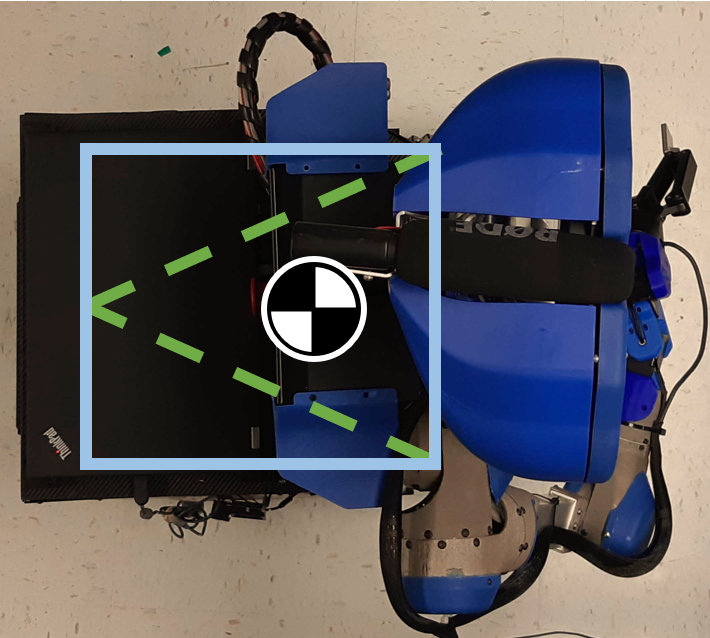
\includegraphics[width=250pt]{images/floor_support.png}
  \caption{Floor support fix}
\end{figure}

\newpage
\section{Software}

\subsection{Natural language understanding using SNIPS}

\tab On previous instances of the Robocup, network issues were causing our speech-to-text solution to misperform significantly. At Robocup 2019, we used a new software called Snips\footnote{\url{https://snips.ai/}}. Snips is an offline speech-to-text (STT) and Natural language understanding (NLU) solution that can be customised to any context. To achieve this, we’ve built a ROS wrapper around SNIPS\footnote{\url{https://github.com/WalkingMachine/wm_snips_asr/blob/fix/ros_integration/src/wm_snips_service.py}} using it’s MQTT API. Since snips is also an NLU framework, it reduces the amount of work needed to combine multiple packages together like we did the year before. It also enhance the quality of the recognition by being context sensitive. As such, we can adjust the expected speech to the situation by switching NLU models.\\

This allowed us to build a proper offline voice interface for our robot. Thus, SNIPS is robust enough to work in remote locations or spaces with poor connectivity like a noisy restaurant. 

\newpage
\subsection{Grasping unknown objects}
\tab Many scenarios involve grasping different objects in a 3D environment. Our approach to achieve this task uses object segmentation\footnote{\url{https://github.com/WalkingMachine/wm_object_segmentation}} coupled with automatic grasp detection.
At first, we detect the table\footnote{\url{https://github.com/WalkingMachine/wm_table_segmentation}} surface and then remove it to keep only the objects.

\begin{figure}
  \centering
  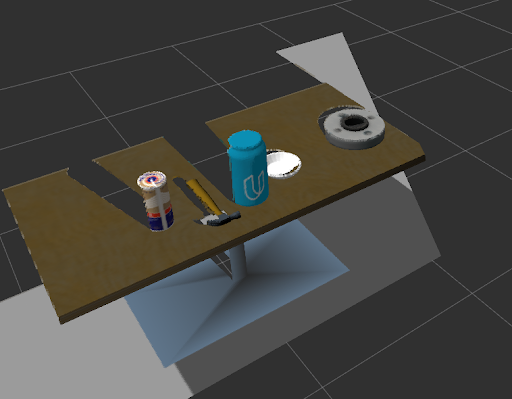
\includegraphics[width=400pt]{images/grasp.png}
  \caption{detection of table with objects }
\end{figure} 

This allow us to extract the outlier objects that pops out. The resulting pointclouds are then passed as inputs to our general object tracker to be identified if possible.

\begin{figure}
  \centering
  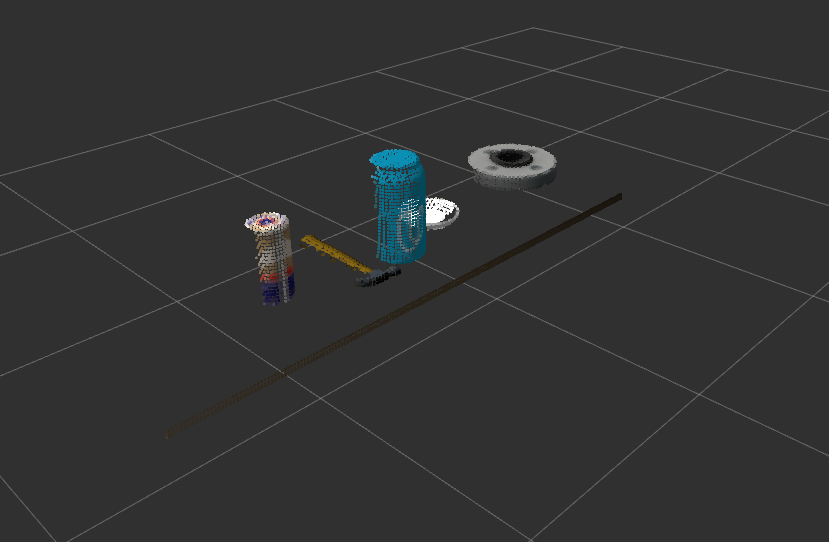
\includegraphics[width=250pt]{images/grasp2.png}
  \caption{empty objects}
\end{figure}

\newpage
\subsection{Grasp pose detection (GPD)}

Once we get the objects, we can start grasping\footnote{\url{https://github.com/WalkingMachine/wm_grasp_selection}} them. The GPD from Andreas ten Pas grasp pose detection\footnote{\url{https://github.com/atenpas/gpd/tree/forward}} is then applied on the segmented pointcloud of the object. Out strategy is to combine GPD with our object detection to clearly identify the desired object to grasp. 
\begin{figure}
  \centering
  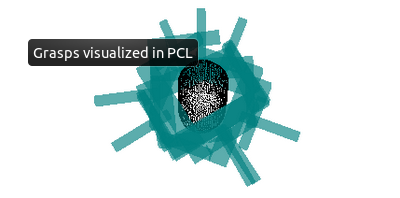
\includegraphics[width=300pt]{images/gpd2.png}
  \caption{Grasps visualized in PCL}
\end{figure}

\newpage
\subsection{Custom dataset generation}

wm\_dataset\_preparation\\

Goal: reduce the time needed to generate a custom dataset for object recognition\\
\begin{itemize}
  \item Motorized platform to easily generate a dataset of every objects from multiple views
  \item Background removal and object isolation using hsv filtering and image processing
  \item New pictures are then generated by pasting the isolated object on given background
  \item Data augmentation is then applied (flip, blur, occlusion...)
\end{itemize}
 
\subsection{Human pose estimation}
\tab Using Openpifpaf\footnote{\url{https://github.com/WalkingMachine/wm_openpifpaf_ros_wrapper}} has drastically increased the recognition of human pose. This will be integrated in many behaviours for the competition. By synchronizing the depth of the camera, we are able to have a 3D output, which also increases the accuracy of the poses. Openpifpaf is also more accurate than OpenPose for partially occluded people.\\

We intend to experiment with classification Algorithms\footnote{\url{https://github.com/WalkingMachine/wm_pose_classification}} to classify the human pose based on joints.\\

With this classification, we are now able to differentiate seated people from standing ones and if either one arm is raised or not. This will drastically improve how we perform during the competition.\\

\newpage
\section{This years goals}

\tab Robocup 2019 allowed us to understand what needed to be improved in our platform and our methods. Participating in stage 2 was a first, but we intend to participate again. For this matter, we will significantly improve our navigation stack to be smoother and faster. We are currently working on simulating our robot on gazebo which will make it easier to test our scenarios.\\
 
We worked hard on the offline mode of our robot, making it independent from any network(internet).We found a local solution to STT and TTS by using SNIPS.\\
 
We are really proud of the physical aspect of SARA, but we would like to make her more understandable for everyone by developing an emotion engine. This will not only enhance her, it will also make it easier to interact with the operator. This interface will show clearly where the robot is in its thought process, helping us debugging her as well as informing the operator of the next step.\\

With these improvements, we hope to be one of the top teams of Robocup 2020.
\newpage
\section*{Robot SARA Hardware Description}
% TODO Change picture and description
Specifications for robot SARA are as follows:

\begin{table}

\label{my-label}

\begin{tabular}{l|p{90mm}}
\hline
\rowcolor[HTML]{FFFFFF} 
\multicolumn{2}{c}{\cellcolor[HTML]{FFFFFF}\textbf{SARA}}                                                      \\ \hline
\rowcolor[HTML]{EAEFF6} 
\textbf{Base}               & Custom base with fully holonomic platform                                        \\
\rowcolor[HTML]{FFFFFF} 
\textbf{Right arm}          & 7 DoF custom arm made of Kinova motors                                           \\
\rowcolor[HTML]{EAEFF6} 
\textbf{Neck}               & Tilt and pan unit using two Dynamixel MX-64R servo actuator                      \\
\rowcolor[HTML]{FFFFFF} 
\textbf{Head}               & Custom head made of RGB neopixels leds and Asus Xtion Pro                        \\
\rowcolor[HTML]{EAEFF6} 
\textbf{Gripper}            & Robotiq 2 fingers 140mm                                                           \\
\rowcolor[HTML]{FFFFFF}
\textbf{Dimensions}         & \begin{tabular}[c]{@{}l@{}}Base : 0,61m. X 0,77m.\\ Height : 1,68m.\end{tabular} \\
\rowcolor[HTML]{EAEFF6} 
\textbf{Weight}             & $\sim$60kg                                                                      \\
\rowcolor[HTML]{FFFFFF} 
\textbf{Additional sensors} & Hokuyo UTM-30LX on base                                                          \\
\rowcolor[HTML]{EAEFF6} 
\textbf{Microphone}         & Rode microphone											                         \\
\rowcolor[HTML]{FFFFFF} 
\textbf{Batteries}          & 2x 20V Dewalt drill battery 5aH                                                 \\
\rowcolor[HTML]{EAEFF6} 
\textbf{Computer}           & 1x Lenovo p50 with 32GB RAM and nVidia Quadro M2000 4GB, 1x Raspberry Pi 3       \\ \hline
\end{tabular}
\caption{Robot's hardware description}
\end{table}
\begin{wrapfigure}[10]{r}{0.25\textwidth}
	\centering
	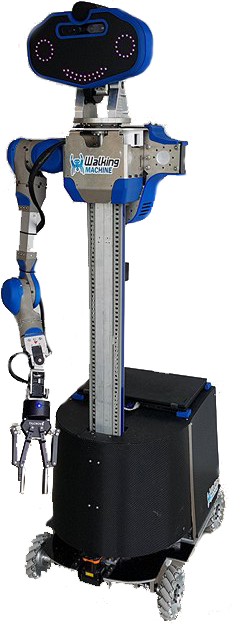
\includegraphics[width=0.30\textwidth]{images/sara_2.png}
	\caption{Robot SARA}
\end{wrapfigure}
\section*{Robot's Software Description}

For our robot we are using the following software:

\begin{itemize}
	\item Platform: Robotic Operating System (ROS) Kinetic on Ubuntu 16.04
	\item Navigation, localization and mapping: \href{http://wiki.ros.org/gmapping}{Gmapping}, \href{http://wiki.ros.org/amcl}{AMCL}, \href{http://wiki.ros.org/pointcloud_to_laserscan}{pointcloud\_to\_laserscan}
	\item Face recognition: \href{http://wiki.ros.org/people}{People}
	\item Speech recognition: \href{https://github.com/WalkingMachine/lab_ros_speech_to_text}{Google Speech API}
	\item Speech comprehension: \href{http://sag.art.uniroma2.it/lu4r.html}{LU4R}, \href{https://github.com/WalkingMachine/lu4r_ros}{lu4r\_ros}
	\item Speech generation: \href{https://doc.ubuntu-fr.org/svoxpico}{Svoxpico}
	\item Object recognition: \href{https://github.com/WalkingMachine/wm_darknet}{Darknet with YOLO v2 }
	\item Arm control: \href{http://wiki.ros.org/moveit}{MoveIt} and \href{https://github.com/Kinovarobotics/kinova-ros}{Kinova API}
	\item Task executor: \href{http://wiki.ros.org/flexbe}{Flexbe} 
	\item World reprensentation: \href{http://github.com/walkingmachine/wonderland}{Wonderland}
\end{itemize}
\bibliographystyle{plain}
\bibliography{references}

Table and object segmentation : 

\url{https://snips.ai/}

\url{https://github.com/WalkingMachine/wm_snips_asr/blob/fix/ros_integration/src/wm_snips_service.py}

\url{https://github.com/WalkingMachine/wm_table_segmentation}

\url{https://github.com/WalkingMachine/wm_object_segmentation} \\

GPD Package :

\url{https://github.com/WalkingMachine/wm_grasp_selection}

\url{https://github.com/atenpas/gpd/tree/forward}

\url{https://www2.ccs.neu.edu/research/helpinghands/code.html} \\

Pose estimation :

\url{https://github.com/WalkingMachine/wm_openpifpaf_ros_wrapper}

\url{https://github.com/WalkingMachine/wm_pose_classification} \\

\section*{Team members}

\begin{tabular}{lll}
   
Olivier Allard &    & 	Automated manufacturing engineering bachelor student \\
André-Philippe Audette &    & 	Electrical engineering bachelor student \\
Nicolas Bernatchez &    & 		Automated manufacturing engineering bachelor student \\
Jeffrey Cousineau &    & 		Automated manufacturing engineering bachelor student (veteran) \\
Simon Desautels &    & 		Software engineering bachelor student \\
Raphaël Duchaîne &    & 		Software engineering bachelor student \\
Gary Grutzner &    & 	Operations and logistics engineering bachelor student \\ 
Nicolas Handfield &    & 	Technological academic path to engineering bachelor student \\ 
Ngoc Phuong Thao Hoang &    & 	Automated manufacturing engineering bachelor student \\ 
Philippe La Madeleine &    & 	Automated manufacturing engineering bachelor student \\ 
Huynh-Anh Le &    & 			Automated manufacturing engineering bachelor student \\
Alexandre Mongrain  &    & 		Manufacturing engineering bachelor student \\
Minh-Van Ngo  &    & 		Automated manufacturing engineering bachelor student \\
Jimmy Poirier &    & 			Electrical engineering bachelor student \\
Judith Poirier &    & 			Technological academic path to engineering bachelor student \\

\end{tabular}
\end{document} 
